\chapter{Tradução de ROBO para CSP}
\label{chap:cap3}
A Seção 3.1 descreve como foi realizado o processo de tradução automático de ROBO para CSP através do framework Spoofax. Desde a fase inicial da definição da gramática até a geração de código.

\section{Definição da Linguagem ROBO com Spoofax}
Nesta Seção veremos como ocorrreu todo o processo de definição da linguagem ROBO usando o framework Spoofax, o que inclui a definição da sintaxe e transformação da linguagem com o intuito de gerar código CSP semanticamente equivalente à ROBO. Todo o processo ocorreu de modo prático levando em consideração um exemplo real.

\subsection{Ferramentas e Ambiente de Programação}
O desenvolvimento de um compilador exige uma preparação bem elaborada de todo um ambiente de programação. No caso deste trabalho, foi necessário o uso do ambiente de programação Eclipse juntamente com um plugin do Spoofax. O qual foi essencial para o desenvolvimento da abordagem de tradução automática. O plugin tem todas as depedências para a geração de Árvore de Análise Sintática e transformação de código.

\subsection{Definição da Sintaxe}
Essa é a etapa inicial para a construção do compilador, na qual devemos primeiro definir todos os aspectos sintáticos da linguagem de programação utilizada no ambiente RoboMind. Ou seja, essa etapa deverá ser capaz de considerar os programas escritos na linguagem ROBO e assegurá-los que estão sintaticamente corretos. Para a definição da gramática livre de contexto de ROBO foi utilizado o formalismo SDF3, como já explicado no Capítulo \ref{chap:cap2}. Além de definir a gramática, SDF3 também foi utilizado para definir a sintaxe lexical, como por exemplo, palavras reservadas de ROBO. O principal objetivo dessa etapa a geração de uma Árvore Sintática Abstrata (\textit{Abstract Syntax Tree - AST}, em inglês) dos programas ROBO. Esse produto resultante é de extrema importância para a geração de código CSP através do Stratego.

Para exemplificar todo o processo de compilação, definimos um exemplo de programa em ROBO que resolve um problema específico. O problema definido foi o ``Contando Caixas'', proposto por RoboLab-FURB\ref{add-ref} e adaptamos para esta pesquisa. O objetivo desse problema é propor uma solução para a simulação de um robô capaz de contar caixas espalhadas por diferentes cenários. O problema foi alterado para que exista um parâmetro que determina o lado no qual o robô deverá contar, sendo lado esquerdo ou direito. Na Figura \ref{fig:map} é mostrado um mapa utilizado para a simulação do problema em questão. Nele é possível ver um robô e algumas caixas, duas na linha superior e três na linha inferior. Na figura foi adicionado um ``X'' para indicar a posição final que o robô deverá parar após a execução do programa. Para exemplificar uma simulação, considere que o lado direito foi escolhido como parâmetro, desse modo, o robô deverá percorrer em linha reta contando as caixas à sua direita e ao chegar na posição final mostrará o resultado 3, caso o parâmetro fosse o lado esquerdo, a quantidade de caixas contadas pelo robô seria 2.

\begin{figure}[h]
\centering
\caption{Exemplo de Mapa usado no RoboMind}
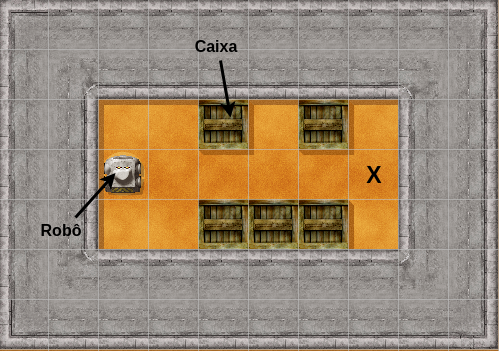
\includegraphics[height=7cm]{figuras/map2.png}
\fonte{O autor}
\label{fig:map}
\end{figure}

Na Figura \ref{fig:roboprogram} está disposto o código de um programa que resolve o problema da contagem de caixas. Esse programa possui duas variáveis globais: (a) \textit{countBoxes}, que é responsável por amazenar a quantidade de caixas; e (b) \textit{lookLine}, que é para indicar qual a linha que o robô deve contar as caixas (esquerda ou direita). Também há um procedimento parametrizado chamado \textit{countLine()}, este possui um único parâmetro denominado \textit{side}, o qual indicará o lado que o robô irá analisar. Se o valor passado ao parâmetro for igual a 1, então contará as caixas do lado esquerdo, se for qualquer valor diferente de 1, então contará as caixas do lado direito. O primeiro movimento do robô ocorre através do comando \textit{right} (indicado na linha 16), o qual altera sua orientação em 90 graus à direita. O próximo passo é a execução de um laço pelo comando \textit{repeatWhile}, a repetição ocorre enquanto não houver quaisquer objetos ou paredes na célula à frente do robô. Esse laço é responsável por chamar o procedimento \textit{countLine()} passando o valor da variável \textit{lookLine}, que neste exemplo tem valor 1, ou seja, contará as caixas da linha esquerda, seguindo de um \textit{forward} que move o robô para frente em uma unidade a cada execução do laço. Ao sair dessa estrutura de repetição, o procedimento será executado mais uma vez, com o objetivo de verificar possíveis caixas na última posição do robô e por fim a quantidade de caixas é exibida por meio do comando \textit{show} exibindo o valor armazenado na variável \textit{countBoxes} contendo a quantidade de caixas na linha de interesse. Este exemplo servirá para toda as etapas, desde a geração de uma AST, após a execução do parser, até a geração de código CSP, após a transformação da árvore.

\begin{figure}[h]
\caption{Programa escrito em ROBO}
\lstinputlisting{codes/program1.rob}
\fonte{O autor}
\label{fig:roboprogram}
\end{figure}

O trabalho \cite{nogueira}, como já mencionado, propõe um compilador que contempla a tradução de programas ROBO sem variáveis e procedimentos. No entanto, a gramática definida resulta uma AST é um formato  \texttt{Program(Sequence, Sequence)} similar a uma tupla, sendo assim, uma limitação, o que impossibilitava o uso de funções do framework Spoofax que facilitassem a transformação da árvore, como por exemplo, aplicação de filtros e recolhimento de termos específicos. Sabendo disso, para facilitar o trabalho em cima da árvore, foi necessário reconstruir partes da gramática de modo que a AST gerada tivesse um formato de lista, assim tornando possível o uso das funções nativas do Spoofax. Na Figura \ref{fig:gramatica_antes} tem um trecho da gramática definida no trabalho citado.

\begin{figure}[h]
\caption{Gramática escrita em forma de sequência}
\lstinputlisting[language=Java]{codes/gramatica_antes.sdf3}
\fonte{O autor}
\label{fig:gramatica_antes}
\end{figure}

Já na Figura \ref{fig:gramatica} a gramática foi totalmente reescrita, antes o que era \texttt{Sequence} tornou-se \texttt{Statement} seguido pelo operador * de concatenação. Dessa forma, ao invés do programa iniciar com uma \texttt{Sequence}, a qual também era seguido por uma \texttt{Sequence} precedida de uma \texttt{Instr}. Além dessa mudança, foi adicionado o termo \texttt{Declaration} (linha 6) que possui três tipos: \texttt{Variable}, \texttt{Procedure} e \texttt{ProcParam} (linhas 8, 9 e 12, respectivamente).

\begin{figure}[h]
\caption{Gramática escrita em forma de lista}
\lstinputlisting[language=Java]{codes/gramatica.sdf3}
\fonte{O autor}
\label{fig:gramatica}
\end{figure}

A definição da sintaxe é composta por módulos que podem ser importados e utilizados em outros módulos. Sabendo disso, o compilador de ROBO foi composto por 4 módulos: (1) \textit{Commom}, contendo toda a parte léxica da linguagem, como restrinções e palavras reservadas; (2) \textit{ExpressionsBoolean}, possuindo todas as definições da gramática para expressões booleanas; (3) \textit{ExpressionsMath}, contém a gramática livre de contexto e as prioridades de análise de cálculo matemático; e (4) \textit{Robo2CSP}, este é o módulo principal, pois engloba os demais, além de definir toda a gramática essencial da linguagem ROBO.

Um programa ROBO consiste em uma lista de declarações (\texttt{Statement}) que podem ser do tipo \texttt{Instr} ou \texttt{Declaration}. O tipo \texttt{Instr} contém todas as instruções básicas de ROBO, ou seja, é composta pelos comandos de movimentação, pintura de mapa, caputura de objetos e as estruturas condicionais e de repetição. Já o tipo \texttt{Declaration} é combinado de declarações para variáveis e para a declaração de procedimentos parametrizados e não parametrizados. Assim, está disposto na Figura \ref{fig:gramatica} parte do módulo Robo2CSP, nela estão definidas as produções da linguagem.

A produção \texttt{Statement.Declaration} define três alternativas para o tipo Declaration que estão definidas em três produções separadas, a primeira \texttt{Declaration.Varia\-ble}, para representar as variáveis, a segunda é \texttt{Declaration.Procedure}, para representar os procedimentos não parametrizados e por fim, \texttt{Declaration.ProcParam}, para representar elementos sintáticos de procedimentos parametrizados.

O corpo da produção para variáveis \texttt{<<Identifier> = <Expr>>} define uma declaração do tipo \texttt{Variable} composta de um identificador (\texttt{Identifier}), que é basicamente um texto descrevendo o nome da variável, seguido por um simbolo de igual e terminado por uma expressão que podem ser do tipo booleanas ou matemáticas (indicadas nas linhas 31 e 32 da Figura \ref{fig:gramatica}, respectivamente).

Para os procedimentos há duas produções, a primeira é para os procedimentos não parametrizados (\texttt{<proce\-dure <Identifier>\{ <Statement*> \}>}) que é composto pela palavra reservada \textit{procedure}, seguido por um identificador, que por sua vez é seguido por zero ou mais \texttt{Statement} entre um par de abre-fecha chaves. Já o segundo, para os procedimentos parametrizados, exige uma complexidade maior, uma vez que um procedimento pode ter \textit{n} parâmetros. A diferença do corpo (\texttt{<procedure <Identifier> <Params> \{ <Statement*> \}}) da produção desse tipo para o corpo do procedimento não parametrizado está na existência da produção \texttt{Params} (linha 28 da Figura \ref{fig:gramatica}) logo após o identificador. O corpo de \texttt{Params} é composto por zero ou mais identificadores separados por vírgula dentro dos símbolos de abre-fecha parênteses.

Uma vez definida as produções para declaração de procedimento, agora é necessário a definição de produções para chamada do mesmo. Esta produção está indicada na linha 34 da Figura \ref{fig:gramatica}. Uma chamada de procedimento nada mais é do que um subtipo de \texttt{Instr}, chamado de \texttt{ProcCall}. O corpo desta produção é composto por um identificador seguido pelos parâmetros, os quais são derivados de expressões. Por isso foi definido um novo tipo de produção, chamado de \texttt{ExprParams} que são \textit{n} expressões separadas por vírgula, entre um par de abre-fecha parênteses.

Descrito o passo a passo de como foi definida a gramática da linguagem ROBO. Agora, entra a etapa do \textit{parsing}, ou seja, o compilador consegue ler um programa escrito em ROBO e gerar sua Árvore Sintática Abstrata com todos os elementos do programa de modo estruturado. Consederando o programa ROBO mostrado na Figura \ref{fig:roboprogram}, geramos a sua AST após a execução do \textit{parsing}. A árvore está denotada pelas Figuras \ref{fig:ast1} e \ref{fig:ast2}, a primeira representa o programa, e a segunda representa o contéudo representado por reticências da linha 4 da figura anterior.

\begin{figure}[h]
\centering
\caption{Geração da AST do programa ROBO}
\lstinputlisting[language=Java]{codes/ast2.aterm}
\fonte{O autor}
\label{fig:ast1}
\end{figure}

\begin{figure}[h]
\centering
\caption{Geração de uma AST do procedimento \textit{countLine()}}
\lstinputlisting[language=Java]{codes/ast1.aterm}
\fonte{O autor}
\label{fig:ast2}
\end{figure}

A geração da AST é essencial para a etapa de geração de código através do Stratego. O Stratego precisa de uma uma árvore como entrada em um formato que facilite sua análise, por isso que as ASTs são representadas em um formato textual, como visto anteriormente. Esse formato é denominado de Formato de Termo Anotado (\textit{Annotated Term Format - ATerm, em inglês}) e cada elemento da árvore é chamado de \textit{Term}. Sabendo disso, a próxima Seção descreve o passo a passo de como é realizada a análise da árvore e como foram definidas as regras de compilação para a geração de código CSP em cima dos \textit{ATerms}.

\subsection{Transformação com Stratego}

Essa etapa é a mais importante, em razão de que o resultado deste processo é o código CSP, produto essencial para a verificação dos programas ROBO semanticamente equivalentes à ROBO no verificador de modelos FDR.

O primeiro passo foi definir uma regra em Stratego para manipular os principais termos de um AST. No qual, para cada termo, outras regras são aplicadas, isto é, o conjunto resultante de termos aplicados à uma regra é utilizado pela regra consecutiva. Isto é melhor exemplificado na regra definida na Figura \ref{fig:rules}. A regra \texttt{main-to-csp} é reponsável por aplicar um cabeçalho para os programas em CSP e desencadear outras regras para os demais termos da árvore. Como a AST de ROBO sempre inicia com \texttt{Program}, isso siginifica que toda geração de código é iniciada por essa regra, no caso ocorre o casamento com o termo \texttt{Program(T1)}, indicado na linha 4, onde \texttt{T1} é todo o restante da árvore sintática. Diante disso, todas as demais regras são aplicadas aos termos derivados de \texttt{T1}.

\begin{figure}[h]
\centering
\caption{Regra inicial para um programa ROBO}
\lstinputlisting{codes/rules.str}
\fonte{O autor}
\label{fig:rules}
\end{figure}

Antes de arbordar sobre as demais partes da regra, vale salientar que o modelo formal de ROBO, especificados em CSP, proposto por \cite{nogueira} possui um processo que simula uma memória devido à impossibilidade de utilizar variáveis em CSP. Por isso, esse processo é utilizado para armazenar apenas os valores da posição (x,y) do robô, sua orientação e a posição (x,y) de um determinado objeto no mapa que são consultados e atualizados em tempo de execução. Diante disso, este trabalho vai reutilizar esta mesma memória para armazenar os valores das variáveis encontradas em programas ROBO, bem como os valores dos parâmetros dos procedimentos. No entanto, na espeficicação formal do trabalho citado anteriormente, os valores dos atributos do robô, citados neste parágrafo, são representados por um conjunto de dados, no formato de chave e valor, para inicialização da memória: \texttt{INIT = \{ (X, startX), (Y, startY), (ORIENTATION, NORTH\_), (BX, startBX), (BY, startBY) \}}. Assim, propomos neste trabalho uma abordagem para que todas as variáveis presentes em programas ROBO sejam adicionadas à esse conjunto \texttt{INIT}. Por exemplo, as variáveis \texttt{countBoxes} e \texttt{lookLine} do programa ilustrado na Figura \ref{fig:roboprogram} seriam adicionadas ao conjunto da seguinte forma: \texttt{INIT = \{ (countBoxes, 0), (lookLine, 1), (X, startX), (Y, startY), (ORIENTATION, NORTH\_), (BX, startBX), (BY, startBY) \}}. 

Sabendo disso, como visto na Figura \ref{fig:rules}, está definida a regra \texttt{main-to-csp} na qual o conteúdo que está entre as linhas 5 e 13 será transformado em código CSP. A linha 5 contém o elemento \texttt{vars'} que é utilizado para transformar todas as variáveis de ROBO em constantes no código CSP. Esse elemento é transformado após a palavra \texttt{with}, no qual outras duas regras são aplicadas em \texttt{T1} e o valor resultante é aplicado a \texttt{vars'}. Inicialmente é aplicado a regra \texttt{<get-vars>} em \texttt{T1}, essa regra tem como objetivo filtrar o conjunto de \textit{ATerms} que casam com o termo \texttt{Declaration(Variable(\_,\_))}, olhar linha 6 da Figura \ref{fig:rules2}. Após isso, uma lista com todos os termos desejados são aplicados na regra mais a esquerda, \texttt{<var-analyze-global>}, que é encarregada de escrever as variáveis declaradas no programa ROBO em forma de constantes na especificação formal CSP. A Figura \ref{fig:rules_constants} mostra a definição das regras responsáveis pela geração das constantes. A regra \texttt{<var-analyze-const>} é aplicada de modo recursivo, muito similar às funções de linguagens funcionais, no qual uma função é aplicada na cabeça (\textit{head}) enquanto a mesma função é aplicada na calda (\textit{tail}) até chegar no caso base, que neste é caso é uma lista vazia, como está indicado na linha 3. A análise ocorre em cima do termo \textit{Declaration(var)}, onde a regra \texttt{<write-variable-const>} é aplicada em \texttt{var} para escrever o CSP correspondente ao tipo de dado da variável. Por isso, há três declarações dessa regra, a primeira para escrever um texto vazio em casos de expressões matemáticas, já que as constantes não recebem expressões (exemplo, a + b); a segunda para escrever o texto \texttt{[name]Const = [v]}, ou seja, o nome da variável (\texttt{name}) e seu respectivo valor inteiro (\texttt{v}); por último, para expressões booleanas, onde uma outra regra, \texttt{<to-csp-e>}, é aplicada para escrever o valor booleano (\textit{true} ou \textit{false}), dependendo do valor do termo em \texttt{exp'}.

\begin{figure}[h]
\centering
\caption{Regras para geração de constantes em CSP}
\lstinputlisting{codes/rules_constants.str}
\fonte{O autor}
\label{fig:rules_constants}
\end{figure}

Outro ponto a destacar está na linha 6 da Figura \ref{fig:rules}, no qual \texttt{MAXVAR} indica os limites inferior e superior que as variáveis poderão antigir durante a execução do programa em FDR, pois em CSP se o conjunto númerico for muito grande, a verificação poder ter o desempenho comprometido devido a grande quantidade de estados que o programa possui. Ainda em relação as variáveis, está declarado na linha 7, o tipo de dados \texttt{VarType}, que em CSP atribui os tipos dos parâmetros (\texttt{paramsType'}) e das variáveis (\texttt{varsType'}) encontrados nos programas ROBO.

\begin{figure}[h]
\centering
\caption{Conjunto de regras auxiliares}
\lstinputlisting[language=Java]{codes/rulesAux.str}
\fonte{O autor}
\label{fig:rules2}
\end{figure}

Para gerar código CSP em relação ao tipo de dados para parâmetros e variáveis através dos elementos \texttt{paramsType'} e \texttt{varsType'} é necessário aplicar algumas regras para recolher os termos de interesse na árvore sintática. A primeira regra aplicada ocorre em \texttt{paramsType'}, ver linha 8 da Figura \ref{fig:rules2}. A regra \texttt{<get-params>} aplica uma função nativa do \textit{Stratego}, chamada de \texttt{collect-all}, cujo objetivo é recolher todos os termos por meio de uma busca por toda árvore AST, o que inclue os nós e seus respectivos filhos. O retorno dessa função é uma lista contendo todos os termos \texttt{Params(\_)} do programa ROBO que, em seguida,  é aplicada à regra \texttt{<get-ids>} que de modo similar a regra anterior recolhe todos os termos contendo os identificadores (\texttt{ID(\_)}) dos parâmetros. Após todo esse processo de filtragem de termos, ocorre a escrita de texto, ou seja, o código CSP é gerado. Na Figura \ref{fig:rules_param_type} está destacada a implementação da regra \texttt{<param-analyze-type>} que é aplicada na lista gerada após a aplicação da regra \texttt{<get-ids>}, como foi bem colocado.

Essa regra é aplicada também de modo recursivo, a recursão ocorre na linha 4, onde o primeiro elemento da lista \texttt{ID(n)} é analisado e destinado a regra \texttt{<write-param\-type>} que é aplicada em \texttt{n}, enquanto para o restante da lista (\texttt{es}) a regra principal é aplicada recursivamente. A regra \texttt{write-param-type} escreve o código CSP, todo o contéudo que está entre os síbmbolos crifrão e colchetes é convertido em texto e \texttt{[n]} é substituído pelo nome do parâmetro analisado. Para exemplificar, o termo \texttt{ID("side")}, visto na linha 4 da Figura \ref{fig:ast2}, é escrito em CSP como \texttt{side.MAXVAR} após todo esse processo descrito, o mesmo vale para todos os parâmetros em qualquer código ROBO.

\begin{figure}[h]
\centering
\caption{Regras para os tipos de dados de parâmetros em código CSP}
\lstinputlisting[language=Java]{codes/rules_param_type.str}
\fonte{O autor}
\label{fig:rules_param_type}
\end{figure}

De modo semelhante ao que é feito em \texttt{paramsType'}, também ocorre em \texttt{vars\-Type'}. A diferença está em como ocorre a escrita de código CSP, uma vez que as variáveis ROBO possuem dois tipos de dados em suas expressões: \texttt{Bool}, para expressões com valores booleanos e \texttt{MAXVAR}, para expressões com valores inteiros. A regra \texttt{<write-variable-type>}, como mostra nas linhas 6 e 9 da Figura \ref{fig:rules_var_type}, aparece duas vezes, a primeira para termos que possuem expressões matemáticas e a segunda para os termos com expressões booleanas.

\begin{figure}[h]
\centering
\caption{Regras para os tipos de dados de variáveis em código CSP}
\lstinputlisting[language=Java]{codes/rules_var_type.str}
\fonte{O autor}
\label{fig:rules_var_type}
\end{figure}

Foi explicado alguns paráfragos antes, que em CSP é necessário um processo para simular uma mémória que armazena os valores das variáveis e demais dados do robô. Assim, a escrita do CSP de parâmetros e variáveis em \texttt{INIT}, através dos elementos \texttt{paramsInit'} e \texttt{varsInit'}, ocorre de modo análago as explicações dadas para os tipos de dados de parâmetros e variáveis.

Voltando para a regra principal, \texttt{<main-to-csp>}, na Figura \ref{fig:rules} está definido o elemento \texttt{proc'} na linha 10, ele é responsável expressar todos os procedimentos dos programas ROBO em um formato compatível com os processos em código CSP, mas que sejam semanticamente iguais ao procedimento escrito na liguagem ROBO. Na linha 21 dessa imagem é possível ver que há a regra \texttt{<union>}, ela é uma regra nativa do framework, cujo objetivo é aplicar o conceito matemático de união de conjuntos em duas listas. Como existem dois tipos de procedimentos na linguagem ROBO, os parametrizados e não parametrizados, é necessário aplicar individualmente duas regras em \textit{T1} para recolher todos os termos relacionados aos procedimentos (olhar linhas 3 e 4 da Figura \ref{fig:rules2}) e depois combiná-las em uma única lista. Essa lista resultante é aplicada na regra \texttt{<statement-definition-decl>}, exposta na Figura \ref{fig:rules_proc}.

\begin{figure}[h]
\centering
\caption{Regras para a geração de código CSP dos procedimentos}
\lstinputlisting[language=Java]{codes/rules_proc.str}
\fonte{O autor}
\label{fig:rules_proc}
\end{figure}

Para essa regra também é preciso de recursividade, uma vez que devemos aplicar algumas regras para cada procedimento na lista. A escrita de código CSP ocorre na regra \texttt{<to-csp>} que é aplicada ao conteúdo de \texttt{s} no termo \texttt{Declaration(s)}. Se \texttt{s} casar com a estrutura \texttt{ProcParam(ID(name), Params(params), procedureBody}, então a geração do código deve ocorrer. Sendo \texttt{name} o nome do procedimento; \texttt{params} a lista de parâmetros; e \texttt{procedureBody} as instruções dentro do corpo do procedimento. Em CSP um processo foi definido como o nome do procedimento em ROBO com a junção do sufixo \texttt{Proc} seguido dos parâmetros (\texttt{params'}) e o símbolo de igual, logo em seguida tem o elemento \texttt{paramVar'} seguido de \texttt{procedureBody'}. Para o elemento paramVar' é aplicada a regra <put-param-mem>, implementada com o objetivo de resolver o problema de atualização de valor dos parâmetros, pois em ROBO é possível atualizar o valor do parâmetro a qualquer momento dentro um procedimento. Em tal caso, foi proposta uma abordagem onde cada parâmetro de um procedimento é adicionado à memória antes das instruções de um mesmo procedimento. A Figura \ref{fig:put_proc} destaca as regras responsáveis por isso, o código CSP é gerado na linha 4. Por exemplo, na Figura \ref{fig:roboprogram} tem o parâmetro \texttt{side} no procedimento \texttt{countLine}, então quando o CSP é gerado esse parâmetro é chamado de \texttt{sideParam} e o seu valor é adicionado na memória da seguinte maneira: \texttt{set.side!(sideParam)}.

\begin{figure}[h]
\centering
\caption{Regras que adicionam os valores dos parâmetros na memória em uma chamada de procedimento}
\lstinputlisting[language=Java]{codes/put-var-proc.str}
\fonte{O autor}
\label{fig:put_proc}
\end{figure}

Como passo seguinte, ocorre a geração de código para o corpo do procedimento, onde um procedimento poder conter diferentes instruções, seja para movimentar robô ou chamar inclusive outro procedimento, além de todas as estruturas condicionais e de repetição. Ainda na Figura \ref{fig:rules_proc}, o elemento \texttt{procedureBody'} é aplicado na regra \texttt{<statement-definition>}, explicitado na Figura \ref{fig:statement}. Essa regra aplica recursivamente a regra \texttt{<to-csp>} para todos os termos da lista, quando chegar ao caso base, ou seja, chegou no fim de um procedimento, é escrito a palavra \texttt{SKIP}, um evento necessário em CSP para indicar que algum outro evento terminou.

\begin{figure}[h]
\centering
\caption{Regras que aplica \texttt{to-csp} para cada instrução}
\lstinputlisting[language=Java]{codes/rules_statement.str}
\fonte{O autor}
\label{fig:statement}
\end{figure}

A regra \texttt{<to-csp>} possui múltiplas definições, pois a maioria das outras regras aplicam \texttt{<to-csp>} nos seus termos. Isso ocorre porque existem diferentes tipos de instruções, algumas delas estão representadas na árvore mostrada na Figura \ref{fig:ast1}, como por exemplo, \texttt{ProcCall} e \texttt{SHOW}. Na Figura \ref{fig:to_csp} está destacada essas duas regras, a primeira, representada da linha 3, gera o código CSP para ocorrência de chamada de procedimento, enquanto a segunda regra, linha 13, expressa a geração de código CSP do comando que exibe valores no \textit{console}, que neste caso gera código CSP para exibir valores inteiros, mas existe uma outra regra \texttt{<to-csp>} para gerar código que exibe valores booleanos.

\begin{figure}[h]
\centering
\caption{Exemplos da regra \texttt{to-csp}}
\lstinputlisting[language=Java]{codes/to-csp.str}
\fonte{O autor}
\label{fig:to_csp}
\end{figure}

Todas as instruções de um programa ROBO são adicionadas dentro do processo chamado de \texttt{COMMANDS} em CSP onde todas instruções são representadas pelo elemento \texttt{instr'} indicado na linha 22 da Figura \ref{fig:rules}. Como o foco deste trabalho são as regras para procedimentos e variáveis, serão explicadas apenas as definições de \texttt{<to-csp>} que representam instruções dessa natureza. A primeira deverição de \texttt{<to-csp>} é para chamada de procedimentos que está definida na Figura \ref{fig:to_csp}. Nela foi proposto uma abordagem para antes de uma chamada de procedimento, em CSP, deve-se obter os valores das variáveis atualizados, mostrado na linha 5, que é representado pelo elemento \texttt{vars'}. Para esse elemente é aplicada a regra \texttt{<get-vars-exp>} com o objetivo de recolher todas as variáveis presentes na expressão (\texttt{ExprParams()}). Depois é aplicada a regra \texttt{<put-get-var-exp-analyze>}, cujo objetivo é colocar todas as variáveis no formato reconhecido CSP, como mostra na Figura \ref{fig:rules_var}. Na linha 6 ocorre a escrita do texto CSP pela regra \texttt{<put-get-var-exp>}, por exemplo, em um caso prático, a variável \texttt{countBoxes} em ROBO seria escrita como \texttt{get.countBoxes?countBoxesVar} no modelo formal. Já para escrever os parâmetros é aplicada a regra  \texttt{<get-param-names-call>} nos termos de \texttt{params}, lembrando que quando ocorre uma chamada de procedimento é possível passar variáveis, valores e expressões como parâmetro. Na Figura \ref{fig:rules_param} mostra várias definições dessa regra, uma vez que há expressões matemáticas e booleanas, além do mais a aplicação dela ocorre de modo recursivo. Por exemplo, na linha 7, mostra o momento em que é empregada a regra \texttt{<to-csp-e>} para o elemento \texttt{exp'} que tem o propósito de gerar código CSP das expressões. O mesmo argumento é aplicável para as demais derivações dessa regra.

\begin{figure}[h]
\centering
\caption{Regras para gerar paramâteros em uma chamada de procedimento}
\lstinputlisting[language=Java]{codes/rules_proc_call.str}
\fonte{O autor}
\label{fig:rules_param}
\end{figure}

\begin{figure}[h]
\centering
\caption{Regras para buscar e atualizar valores das variáveis}
\lstinputlisting[language=Java]{codes/rules_var.str}
\fonte{O autor}
\label{fig:rules_var}
\end{figure}

Outra versão de \texttt{<to-csp>} foi definida para atualização de variáveis, indicada pela linha 10 na Figura \ref{fig:rules_var}. Na linha 12 é possível notar quando o código CSP é gerado com intuito de escrever uma consulta do valor da própria variável, enquanto as demais variáveis são representadas pelo elemento \texttt{var'}, na linha 13. Essa abordagem é necessária porque uma variável pode ser atualizada pelo usando ela mesma, além de uma combinação de expressões com diferentes variáveis e valores. O código CSP da atualização do valor dela na memória ocorre na linha 14. Para fins práticos, considerando a expressão \texttt{countBoxes = countBoxes + 1}, ela seria escrita em CSP como \texttt{member((countLineVar + 1), MAXVAR) \& set.countLine!((countLineVar + 1))}. Isso quer dizer que primeiro é verificado se o novo valor da variável está dentro do limite inferior e superior para que de fato seja atualizada pelo comando \texttt{set}.

Em vista das explicações mencionadas à respeito das regras de tradução implementadas para procedimentos e variáveis, entende-se que de agora em diante é possível gerar código CSP automaticamente para programas ROBO. A tradução é contemplada com as regras de compilação iniciais apresentadas em \cite{nogueira} para as instruções básicas do robô, agora também incluem regras para programas que possuem declarações de procedimentos e variáveis e chamadas de procedimentos e atualizações de variáveis.

